\clearpage
\genHeader

\subsection{A first look at EA}

\begin{itemize}
\FloatBarrier
\hypertarget{simpleDemo vis}{}
\item[$\blacktriangleright$] Can you locate the new \texttt{Demo.eap} file in your package explorer? This is the EA project file you'll be
modelling in. Don't worry about any other folders at the moment - all problems will be resolved by the end of this section.

In the meantime, do not rename, move, or delete anything.

\item[$\blacktriangleright$] Double-click \texttt{Demo.eap} to start EA, and choose \texttt{Ultimate} when starting EA for the first time.

\item[$\blacktriangleright$] In EA, navigate to and select ``Extensions/Add-In Windows'' (Fig.~\ref{ea:validate_dropdown}). This will activate our tool's full
control panel.

\vspace{0.5cm}

\begin{figure}[htbp]
	\centering
  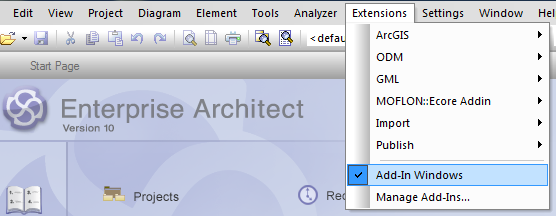
\includegraphics[width=1\textwidth]{ea_extensionMenu}
	\caption{Export from EA} 
	\label{ea:validate_dropdown} 
\end{figure}

\item[$\blacktriangleright$] This tabbed control panel provides access to all of
eMoflon's functionality. This is where you can validate and export your complete project to Eclipse by pressing \texttt{All} (Fig.~\ref{ea:controlPanel}).

\begin{figure}[htbp]
	\centering
  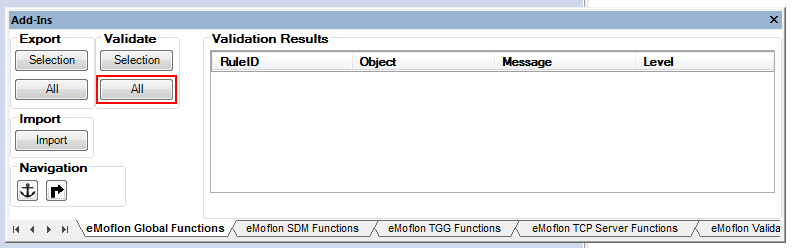
\includegraphics[width=0.9\textwidth]{ea_controlPanelValidateAll}
	\caption{eMoflon's control panel in EA} 
	\label{ea:controlPanel} 
\end{figure}

\item[$\blacktriangleright$] Now try exploring the EA project browser! Try to navigate to the packages, classes, and diagrams. Don't worry if you don't
understand that much - we'll get to explaining everything in a moment. Just make sure not to change anything!

\item[$\blacktriangleright$] Switch back to Eclipse, choose your metamodel project, and press \texttt{F5} to refresh. 
The export from EA places all required files in a hidden folder (.temp) in the project.
A new, third project named \emph{org.moflon.demo.doublelinkedlist} is now being created.
Do not worry about the problem markers.

\item[$\blacktriangleright$] The three asterisks (Fig.~\ref{eclipse:dirty-project}) signal that the project still needs to be built.

\vspace{0.5cm}

\begin{figure}[htbp]
    \centering
    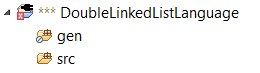
\includegraphics[width=0.35\textwidth]{eclipse_dirtyProject}
    \caption{Dirty projects are marked with ***} 
    \label{eclipse:dirty-project} 
\end{figure}

\vspace{0.5cm}

\item[$\blacktriangleright$] Now, right-click \emph{org.moflon.demo.doublelinkedlist} and choose ``eMoflon/Build" (or use the shortcut Alt+Shift+E,B\footnote{First press Alt+Shift+E, release, and press B.
By default, most shortcuts eMoflon start with Alt+Shift+E.}).

eMoflon now generates the Java code in your repository project.
You should be able to monitor the progress with the green bar in the lower right corner (Fig.~\ref{eclipse:build}). Pressing the
symbol opens a monitor view that gives more details of the build process. You don't need to worry about any of these details, just remember to \begin{inparaenum}[(i.)]
\item refresh your Eclipse workspace after an export, and
\item rebuild projects that bear a ``dirty" marker (\texttt{***}).
\end{inparaenum}

\begin{figure}[htbp]
    \centering
    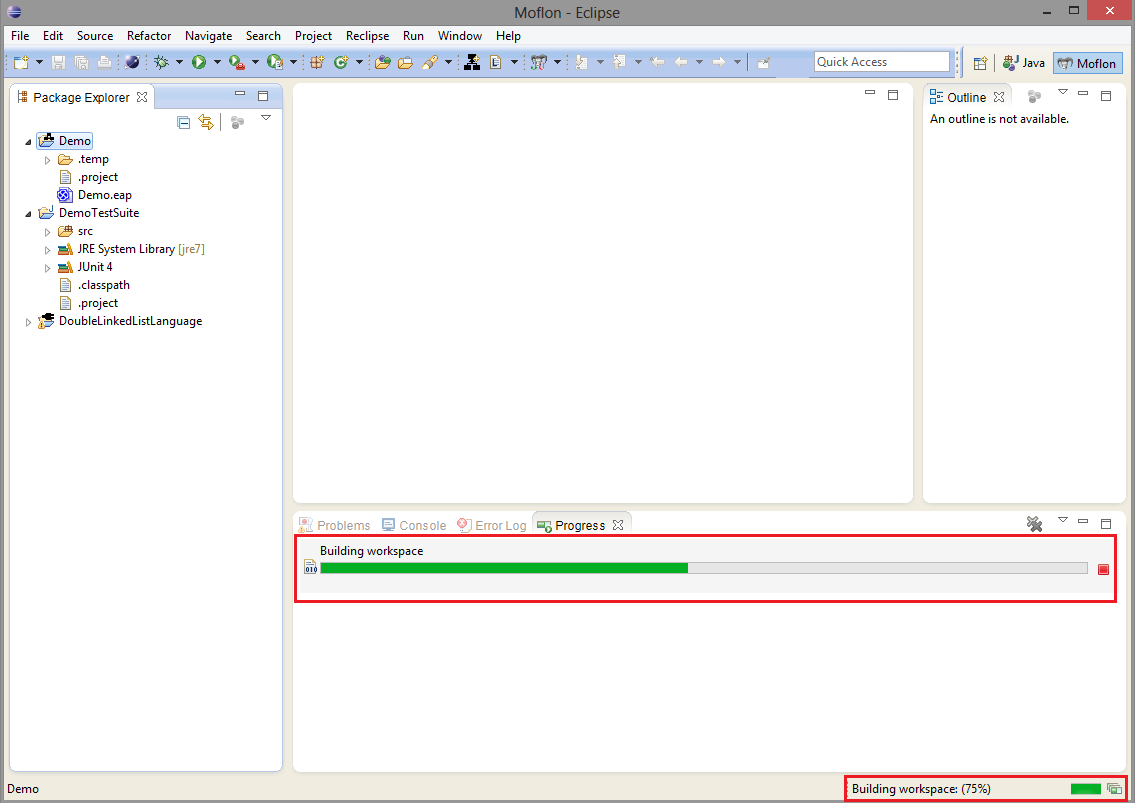
\includegraphics[width=1\textwidth]{eclipse_buildingProgress}
    \caption{Eclipse workspace when using visual syntax} 
    \label{eclipse:build} 
\end{figure}

\item[$\blacktriangleright$] If you're ever worried about forgetting to refresh your workspace, or if you just don't want to bother with having to do this,
Eclipse does offer an option to do it for you automatically. To activate this, go to ``Window/Preferences/General/Workspace" and select \texttt{Refresh on
access}.

\end{itemize}